The immigrant and native populations are different not only in their size but also in their age structure.
By dividing total (across all ages) transfer by the total population, per-capita comparison between immigrant and natives account for the difference in the population size but not for the difference in age structure.
Because public transfers are inter-generational, that is, resources are collected from the working-age population (the outflow transfers) and reallocated to the dependent population, mostly the young and old (the inflows transfers), they are sensitive to the age structure of the population.
Therefore the comparison based on per-capita values is biased to the extent to which the two populations have different age structures.
To account for this difference in age structure, the decomposition discussed earlier is applied to surpluses in each account and sub-account separately.
For a given transfer account, the decomposition function takes as inputs the age-specific transfer and the population size, apply the decomposition algorithm, and returns the two components representing the respective contributions of the inputs to the per crude surplus.
This allows quantifying how much of the crude surplus is due to a difference in age-specific transfer, rather than a  difference in the age structure of the two populations.

\vspace{0.7em}\par
Age-adjusted surpluses are the components associated with the age-specific transfers and represent the difference between an immigrant and a native of the same age.
They are also referred to as fiscal components.
Demographic components on the other hand are associated with the population size and represent the portion of the surplus that results from a difference in the age structure of immigrants and natives populations.
It is important to note that even though the population size is used as inputs, the associated components only reflect the difference in population age structure because the effect of the population size is canceled out in the per-capita calculation.
Also, as Net surplus is the sum of all Immigrant surpluses across all accounts (inflows minus outflow), the age-adjusted Net surplus is computed similarly, as the sum of all age-adjusted Immigrant surpluses. \autoref{fig:DEcomp} presents the trend in the crude and age-adjusted surpluses as well as the demographic components for each sub-accounts throughout the studied period.

\begin{figure}[H]%
  \caption{Trends in Crude, Age-adjusted and demographic components for accounts of inflows and outflows between 1997 and 20/15 }
  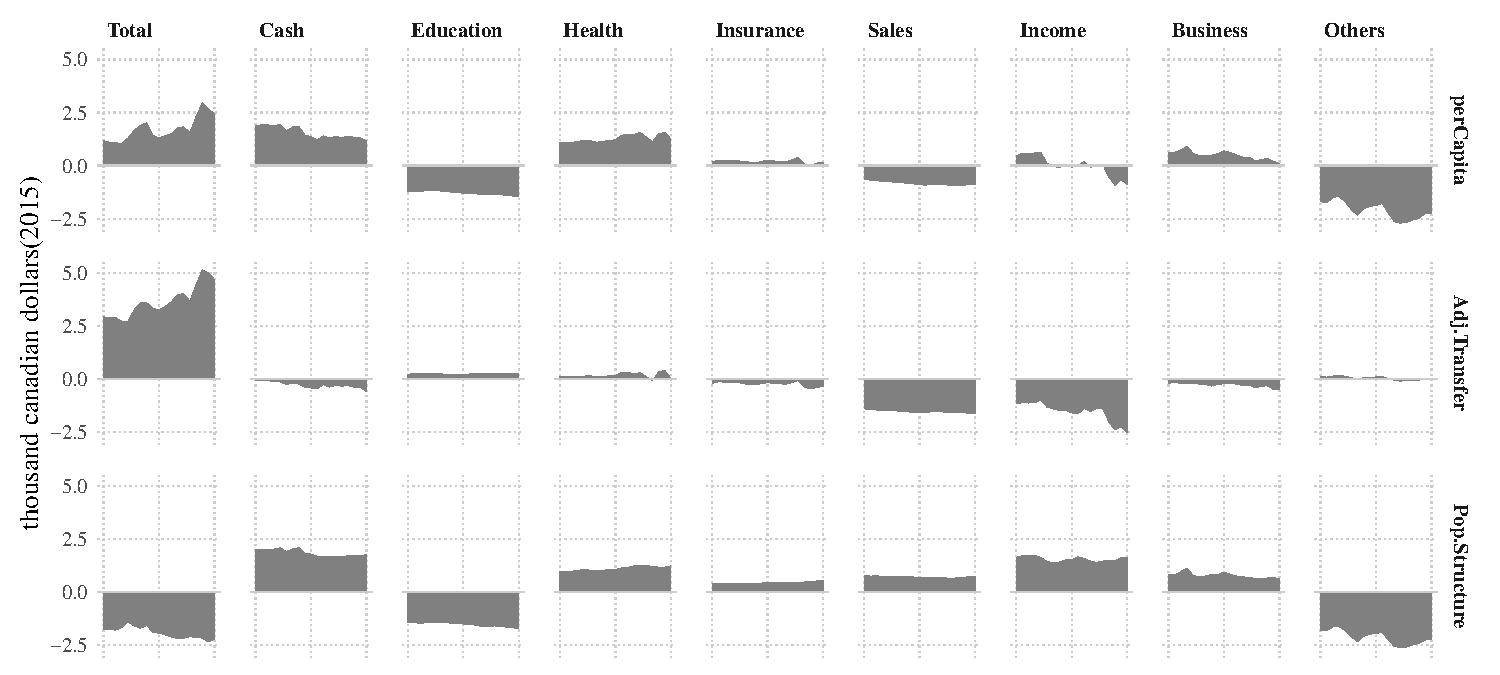
\includegraphics[width=1\textwidth]{res/DEcomp.pdf}%
  \label{fig:DEcomp}%
\end{figure}%

\subsubsection*{Age-adjusted Net surplus}

Results show that age-adjusted Net surplus followed the same pattern as per-capita Net surplus but the levels are much higher in absolute values.
Furthermore, the overall negative sign for demographic components of net surplus indicates that age structure is much favorable to immigrants, as it reduced the difference between immigrant and natives from the adjusted value to the per-capita value.
Put another way, if the immigrants and natives population have had the same age structure, the per-capita difference would have been much higher than its current value.
In dollar value, at equal age, the average immigrant has cost to the state about \DTLfetch{statex}{sKey}{AveAdj.Transfer}{sVal}\$ per year, more than the average native, between 1997 and 2016.
However, a favorable population structure reduced this surplus by about of \DTLfetch{statex}{sKey}{AvePop.Structure}{sVal}\$, leading the  \DTLfetch{statex}{sKey}{AveperCapita}{sVal}\$ in per-capita net surplus.
While the demographic effect has increased steadily during the studied period from \DTLfetch{statex}{sKey}{AvePop.Structure1997}{sVal}\$ to \DTLfetch{statex}{sKey}{AvePop.Structure2015}{sVal}\$, the trends in Adjusted net surplus are much stepping with disruptive increases every few years (early 2000, late 2000, early 2010) from \DTLfetch{statex}{sKey}{AveAdj.Transfer1997}{sVal}\$ in 1997 to \DTLfetch{statex}{sKey}{AveAdj.Transfer2015}{sVal}\$ in 2015.
The steady increase of the demographic components over the years reflects the faster aging of the native population compared to the immigrant population which has been purposefully kept young through various economic immigration programs.

\vspace{0.7em}\par
These results imply that the difference in age structure between immigrant and native populations accounts for much of their difference in crude surpluses.
Therefore, not accounting for the demographic effect leads to conflicting results that confuse our understanding of transfer differential between immigrants and natives, create unnecessary discord in the immigration debates, and lead to inappropriate public policy.
The confusion goes even further when comparing the sub-account of inflow and outflow.


\subsubsection*{Age-adjusted surpluses in sub accounts}

Looking at the adjusted surplus for the sub-accounts, it appears that Income and Sales taxes are the main sources of the net surplus between immigrants and natives.
This is expected, as other sub-accounts being tied to public programs are less likely to increase social inequality such as the one seen in the immigrant surplus.
Income and Sales taxes sub-accounts on the other hand are directly linked to individual revenue on which public policy has less control and therefore are subject to labor market imbalances.
However, this pattern is not observable from the per-capita values.
In fact, trends in the sub-account of crude net surplus show opposite results with inflow sub-accounts appearing as the major sources of disparities in net transfers.
For example, it is intuitive that since most contributions to the public finances are based on a given proportion of the individual's income, income taxes would reflect a large proportion of the difference between immigrants and natives.
On contrary, the crude net surplus for income taxes shows conflicting results being positive between 1997 and 2003, null till 2012, and negative afterward.

\vspace{0.7em}\par
The mitigating effect of demographic components is also illustrated in the high level of the per-capita health care cost which after accounting for the difference in age structure is reduced to close to zero.
This suggests that the per-capita difference in health care cost is largely due to the fact there are relatively more immigrants in the age groups where health care costs are higher.
Demographics not only affect the size of the immigrant surplus but also change its direction and trend.
For example, looking at the per-capita surplus, immigrants seem to have paid on average more business taxes than natives.
The situation reverses after adjusting for demographic effect.
At the same age, not only immigrants pay less in business taxes than natives, but the trend in immigrant surplus is increasing while per-capita measure indicates the opposite.
The low business taxes paid by immigrants suggest that they operate smaller businesses than natives.
They also contributed toward social security and received cash transfers, slightly less than natives.
The opposite applies to education and health care costs where immigrants consume slightly more than natives.

\vspace{0.7em}\par
Other sub-accounts of transfer include public goods and services as well as public deficit and debts.
By design, the NTA method distributes these costs evenly and no difference is expected between immigrants and natives.
This is well reflected in the age-adjusted surplus which is close to zero, the lowest in absolute value among all sub-accounts.
Therefore the large negative effect (in favor of immigrants) seen in the per-capita surplus is mainly due to the difference in age structure between immigrants and natives.
When adjusted for these differences, the surpluses in these other accounts compensated each other, revealing the sub-account of sales and Income taxes as the two most important sources of disparities between immigrants and natives.

\vspace{0.7em}\par
In summary, Immigrants received quite similar benefits from public programs, but their low revenue doesn't allow them to contribute equally to public finances, leading to a surplus in the transfer.
As a result, differences in sales and Income taxes added up to an age-adjusted surplus of \DTLfetch{statex}{sKey}{SIAdjusted}{sVal}\$ which  represent \DTLfetch{statex}{sKey}{SIprop}{sVal}\% of the \DTLfetch{statex}{sKey}{AveAdj.Transfer}{sVal}\$ in total age-adjusted surplus.
As these taxes are deducted from income which is mainly earned from labor, the labor market stands out as the single most important source of inequality between immigrants and natives.
Furthermore, it appears that while both Income and sales taxes are the main contributors to net surplus, Income taxes alone drive its trends.
These results stand against expectations of a positive impact of immigration on public finances, especially for recent immigrants for whom economic factors have motivated the admission.
Therefore understanding how the labor market becomes the source of so much imbalances especially since 2011, is an important and crucial question to discuss and address, should Canada intend to benefits from its immigrants.


















